% Chapter Template

\chapter{Machine Learning} % Main chapter title

\label{Chapter7} % Change X to a consecutive number; for referencing this chapter elsewhere, use \ref{ChapterX}

\lhead{Chapter 2. \emph{Machine Learning}} % Change X to a consecutive number; this is for the header on each page - perhaps a shortened title

%----------------------------------------------------------------------------------------
%	SECTION 1
%----------------------------------------------------------------------------------------

\section{Definition}

Machine Learning is the field of study that gives computers the capability to learn without being explicitly programmed. ML is one of the most exciting technologies that one would have ever come across. As it is evident from the name, it gives the computer that which makes it more similar to humans: The ability to learn. Machine learning is actively being used today, perhaps in many more places than one would expect.

\begin{itemize}
\item Traditional Programming: Data and program is run on the computer to produce the output.
\item Machine Learning: Data and output is run on the computer to create a program. This program can be used in traditional programming.
\end{itemize}
\begin{figure}[htbp]
    \centering
	    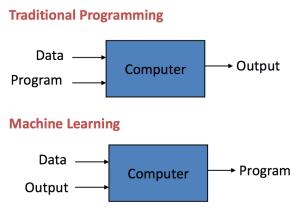
\includegraphics[scale=0.5]{Figures/tl_ml.png}
		    %\rule{10em}{0.5pt}
        \caption[Traditional programming vs Machine Learning]{Traditional programming vs Machine Learning}
	    \label{fig:Traditional programming vs Machine Learning}
\end{figure}
 Machine learning is like farming or gardening. Seeds is the algorithms, nutrients is the data, the gardener is you and plants is the programs.
\clearpage
\section{Types of Machine Learning}

At a high-level, machine learning is simply the study of teaching a computer program or algorithm how to progressively improve upon a set task that it is given. On the research-side of things, machine learning can be viewed through the lens of theoretical and mathematical modeling of how this process works. However, more practically it is the study of how to build applications that exhibit this iterative improvement. There are many ways to frame this idea, but largely there are three major recognized categories:
\begin{enumerate}
    \item Supervised learning
    \item Unsupervised learning
    \item Reinforcement learning
\end{enumerate}

\begin{figure}[htbp]
    \centering
	    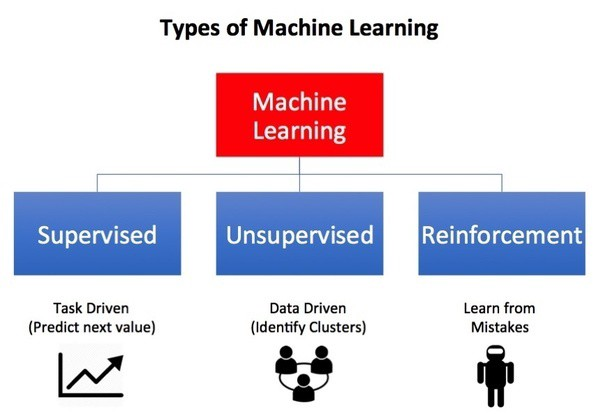
\includegraphics[scale=0.3]{Figures/ml_types.jpg}
		    %\rule{10em}{0.5pt}
        \caption[Types of Machine Learning]{Types of Machine Learning}
	    \label{fig:Traditional programming vs Machine Learning}
\end{figure}

\subsection{Supervised Learning}

Supervised learning is the most popular paradigm for machine learning. It is the easiest to understand and the simplest to implement.\\
Given data in the form of examples with labels, we can feed a learning algorithm these example-label pairs one by one, allowing the algorithm to predict the label for each example, and giving it feedback as to whether it predicted the right answer or not. Over time, the algorithm will learn to approximate the exact nature of the relationship between examples and their labels. When fully-trained, the supervised learning algorithm will be able to observe a new, never-before-seen example and predict a good label for it.

\begin{figure}[htbp]
    \centering
	    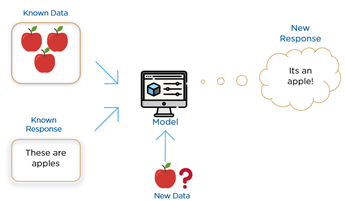
\includegraphics[scale=0.4]{Figures/supervised.png}
		    %\rule{10em}{0.5pt}
        \caption[Supervised Learning]{Supervised Learning}
	    \label{fig:Supervised Learning}
\end{figure}

Supervised Learning uses two types of techniques:

\begin{itemize}
    \item Classification:
        Classification is the process of predicting the class of given data points. Classes are sometimes called as targets/ labels or categories. Classification predictive modeling is the task of approximating a mapping function (f) from input variables (X) to discrete output variables (y).

        For example, spam detection in email service providers can be identified as a classification problem. This is s binary classification since there are only 2 classes as spam and not spam. A classifier utilizes some training data to understand how given input variables relate to the class. In this case, known spam and non-spam emails have to be used as the training data. When the classifier is trained accurately, it can be used to detect an unknown email.

        Classification belongs to the category of supervised learning where the targets also provided with the input data. There are many applications in classification in many domains such as in credit approval, medical diagnosis, target marketing etc.

        There are two types of learners in classification as lazy learners and eager learners.
        \begin{enumerate}
            \item Lazy learners: Lazy learners simply store the training data and wait until a testing data appear. When it does, classification is conducted based on the most related data in the stored training data. Compared to eager learners, lazy learners have less training time but more time in predicting.

            \textit {Ex. k-nearest neighbor, Case-based reasoning}
    
            \item Eager learners: Eager learners construct a classification model based on the given training data before receiving data for classification. It must be able to commit to a single hypothesis that covers the entire instance space. Due to the model construction, eager learners take a long time for train and less time to predict.

            \textit{Ex. Decision Tree, Naive Bayes, Artificial Neural Networks}
    
        \end{enumerate}
        Classification Algorithms:\\
        There is a lot of classification algorithms available now but it is not possible to conclude which one is superior to other. It depends on the application and nature of available data set. For example, if the classes are linearly separable, the linear classifiers like Logistic regression, Fisher’s linear discriminant can outperform sophisticated models and vice versa.
        \begin{itemize}
            \item Decision Tree:
                
                Decision tree builds classification or regression models in the form of a tree structure. It utilizes an if-then rule set which is mutually exclusive and exhaustive for classification. The rules are learned sequentially using the training data one at a time. Each time a rule is learned, the tuples covered by the rules are removed. This process is continued on the training set until meeting a termination condition.
            
            \begin{figure}[htbp]
                \centering
	            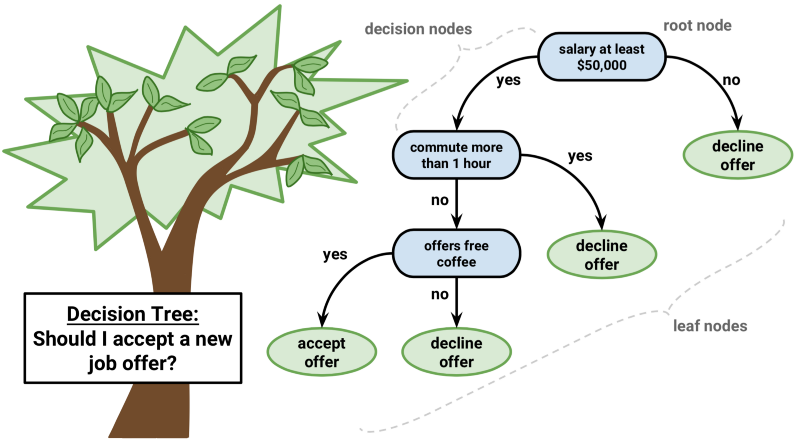
\includegraphics[scale=0.3]{Figures/decision_tree.png}
		        %\rule{10em}{0.5pt}
                \caption[Decision Tree]{Decision Tree}
	            \label{fig:Decision Tree}
                \end{figure}

                The tree is constructed in a top-down recursive divide-and-conquer manner. All the attributes should be categorical. Otherwise, they should be discretized in advance. Attributes in the top of the tree have more impact towards in the classification and they are identified using the information gain concept.

                A decision tree can be easily over-fitted generating too many branches and may reflect anomalies due to noise or outliers. An over-fitted model has a very poor performance on the unseen data even though it gives an impressive performance on training data. This can be avoided by pre-pruning which halts tree construction early or post-pruning which removes branches from the fully grown tree.

        \item Naive Bayes:
                Naive Bayes is a probabilistic classifier inspired by the Bayes theorem under a simple assumption which is the attributes are conditionally independent.\\
                    \begin{figure}[htbp]
                        \centering
	                    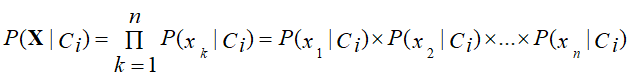
\includegraphics[scale=0.5]{Figures/naive_bayes.png}
		                %\rule{10em}{0.5pt}
                        \caption[Naive Bayes]{Naive Bayes}
	                    \label{fig:Naive Bayes}
                    \end{figure}
                The classification is conducted by deriving the maximum posterior which is the maximal P(Ci|X) with the above assumption applying to Bayes theorem. This assumption greatly reduces the computational cost by only counting the class distribution. Even though the assumption is not valid in most cases since the attributes are dependent, surprisingly Naive Bayes has able to perform impressively.

                Naive Bayes is a very simple algorithm to implement and good results have obtained in most cases. It can be easily scalable to larger datasets since it takes linear time, rather than by expensive iterative approximation as used for many other types of classifiers.

                Naive Bayes can suffer from a problem called the zero probability problem. When the conditional probability is zero for a particular attribute, it fails to give a valid prediction. This needs to be fixed explicitly using a Laplacian estimator.
                
        \item Artificial Neural Networks:
                Artificial Neural Network is a set of connected input/output units where each connection has a weight associated with it started by psychologists and neurobiologists to develop and test computational analogs of neurons. During the learning phase, the network learns by adjusting the weights so as to be able to predict the correct class label of the input tuples.

                \begin{figure}[htbp]
                    \centering
	                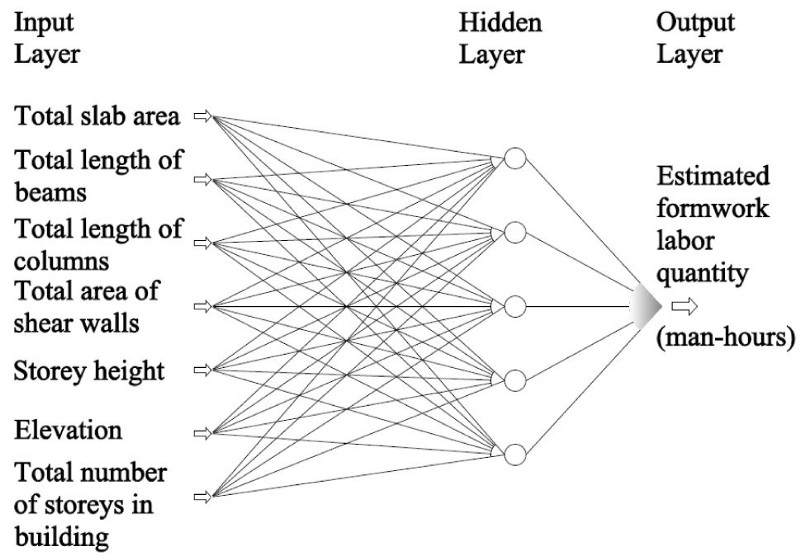
\includegraphics[scale=0.3]{Figures/ann.jpeg}
		            %\rule{10em}{0.5pt}
                    \caption[Artificial Neural Network Design]{Artificial Neural Network Design}
	                \label{fig:Naive Bayes}
                \end{figure}
                
                There are many network architectures available now like Feed-forward, Convolutional, Recurrent etc. The appropriate architecture depends on the application of the model. For most cases feed-forward models give reasonably accurate results and especially for image processing applications, convolutional networks perform better.

                There can be multiple hidden layers in the model depending on the complexity of the function which is going to be mapped by the model. Having more hidden layers will enable to model complex relationships such as deep neural networks.

                However, when there are many hidden layers, it takes a lot of time to train and adjust wights. The other disadvantage of is the poor interpretability of model compared to other models like Decision Trees due to the unknown symbolic meaning behind the learned weights.

                But Artificial Neural Networks have performed impressively in most of the real world applications. It is high tolerance to noisy data and able to classify untrained patterns. Usually, Artificial Neural Networks perform better with continuous-valued inputs and outputs.

        \item k-Nearest Neighbor (KNN):
                \begin{figure}[htbp]
                    \centering
	                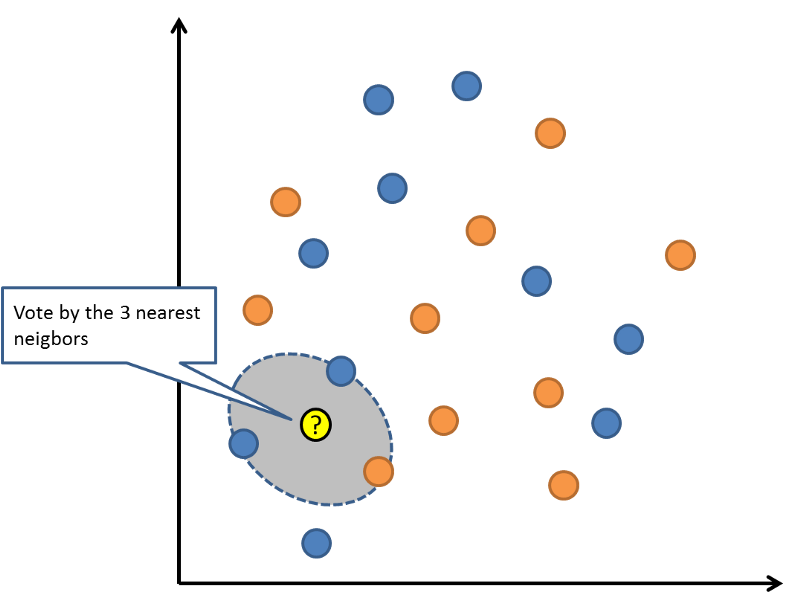
\includegraphics[scale=0.3]{Figures/knn.png}
		            %\rule{10em}{0.5pt}
                    \caption[k-Nearest Neighbor]{k-Nearest Neighbor}
	                \label{fig:Naive Bayes}
                \end{figure}
        
                k-Nearest Neighbor is a lazy learning algorithm which stores all instances correspond to training data points in n-dimensional space. When an unknown discrete data is received, it analyzes the closest k number of instances saved (nearest neighbors)and returns the most common class as the prediction and for real-valued data it returns the mean of k nearest neighbors.

                In the distance-weighted nearest neighbor algorithm, it weights the contribution of each of the k neighbors according to their distance using the following query giving greater weight to the closest neighbors.

                \begin{figure}[htbp]
                    \centering
	                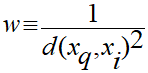
\includegraphics[scale=0.5]{Figures/knn2.png}
		            %\rule{10em}{0.5pt}
                    \caption[Distance calculating query]{Distance calculating query}
	                \label{fig:Naive Bayes}
                \end{figure}
        \end{itemize}
    \item Regression:
                \begin{figure}[htbp]
                    \centering
	                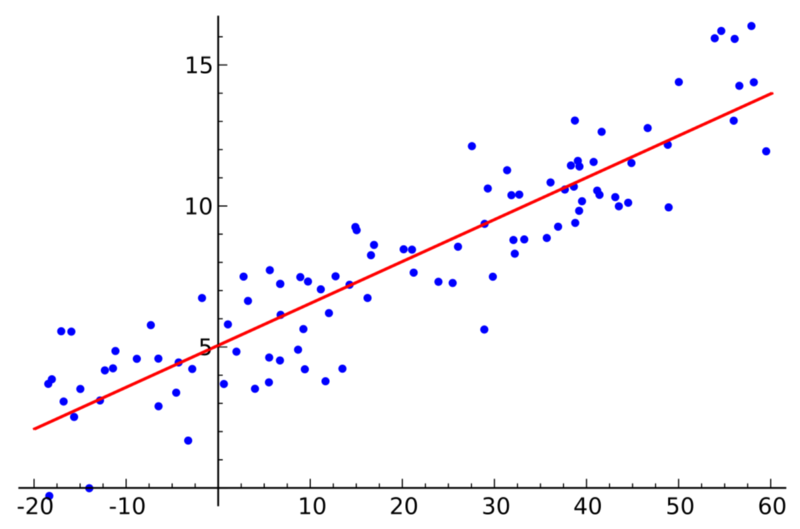
\includegraphics[scale=0.4]{Figures/linear_r.png}
		            %\rule{10em}{0.5pt}
                    \caption[Distance calculating query]{Distance calculating query}
	                \label{fig:Naive Bayes}
                \end{figure}
    
        Simple linear regression is a type of regression analysis where the number of independent variables is one and there is a linear relationship between the independent(x) and dependent(y) variable. The red line in the above graph is referred to as the best fit straight line. Based on the given data points, we try to plot a line that models the points the best. The line can be modelled based on the linear equation shown below.
    
                \begin{figure}[htbp]
                    \centering
	                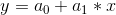
\includegraphics[scale=0.8]{Figures/linear_r1.png}
		            %\rule{10em}{0.5pt}
                \end{figure}
                
        The motive of the linear regression algorithm is to find the best values for a0 and a1. Before moving on to the algorithm, let’s have a look at two important concepts you must know to better understand linear regression.
        
        \clearpage
        Cost Function: The cost function helps us to figure out the best possible values for a0 and a1 which would provide the best fit line for the data points. Since we want the best values for a0 and a1, we convert this search problem into a minimization problem where we would like to minimize the error between the predicted value and the actual value.
        
                \begin{figure}[htbp]
                    \centering
	                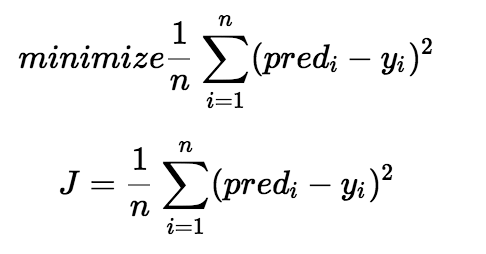
\includegraphics[scale=0.5]{Figures/costfn.png}
		            %\rule{10em}{0.5pt}
		            \caption[Minimization and Cost Function]{Minimization and Cost Function}
	                \label{fig:Minimization and Cost Function}
                \end{figure}
                
        We choose the above function to minimize. The difference between the predicted values and ground truth measures the error difference. We square the error difference and sum over all data points and divide that value by the total number of data points. This provides the average squared error over all the data points. Therefore, this cost function is also known as the Mean Squared Error(MSE) function. Now, using this MSE function we are going to change the values of a0 and a1 such that the MSE value settles at the minima.
        
        Gradient Descent: The next important concept needed to understand linear regression is gradient descent. Gradient descent is a method of updating a0 and a1 to reduce the cost function(MSE). The idea is that we start with some values for a0 and a1 and then we change these values iteratively to reduce the cost. Gradient descent helps us on how to change the values.

                \begin{figure}[htbp]
                    \centering
	                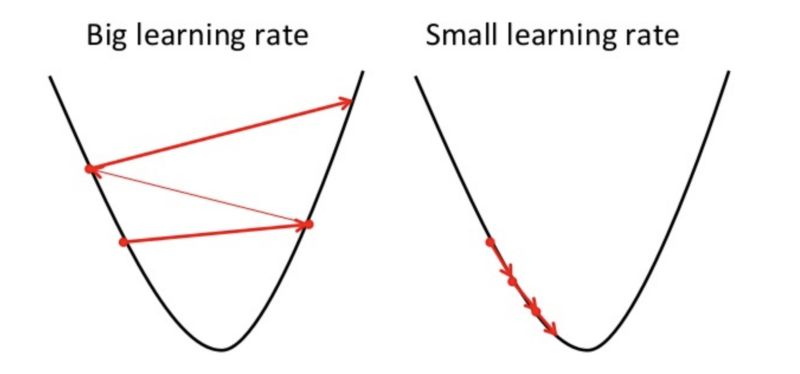
\includegraphics[scale=0.4]{Figures/lrate.png}
		            %\rule{10em}{0.5pt}
		            \caption[Learning Rate]{Learning Rate}
	                \label{fig:Learning Rate}
                \end{figure}
        To draw an analogy, imagine a pit in the shape of U and you are standing at the topmost point in the pit and your objective is to reach the bottom of the pit. There is a catch, you can only take a discrete number of steps to reach the bottom. If you decide to take one step at a time you would eventually reach the bottom of the pit but this would take a longer time. If you choose to take longer steps each time, you would reach sooner but, there is a chance that you could overshoot the bottom of the pit and not exactly at the bottom. In the gradient descent algorithm, the number of steps you take is the learning rate. This decides on how fast the algorithm converges to the minima.
    
\end{itemize}
\subsection{Unsupervised Learning}
    Unsupervised Learning is a class of Machine Learning techniques to find the patterns in data. The data given to unsupervised algorithm are not labelled, which means only the input variables(X) are given with no corresponding output variables. In unsupervised learning, the algorithms are left to themselves to discover interesting structures in the data.